\normaltrue \difficilefalse \tdifficilefalse
\correctionfalse
%\UPSTIidClasse{11} % 11 sup, 12 spé
%\newcommand{\UPSTIidClasse}{11}

\exer{Système éclipse $\star$ \label{C2:04:65:02}}
%% CCP MP 2007
\setcounter{numques}{0}
\UPSTIcompetence[2]{C2-04}
\index{Compétence C2-04}
\index{Correcteur}
\index{Correcteur intégral}
\index{Système éclipse}


\ifcorrection
\else
\textbf{Pas de corrigé pour cet exercice.}
\fi

Le schéma-blocs sous la forme suivante avec un gain unitaire pour le capteur
de vitesse.

\begin{center}
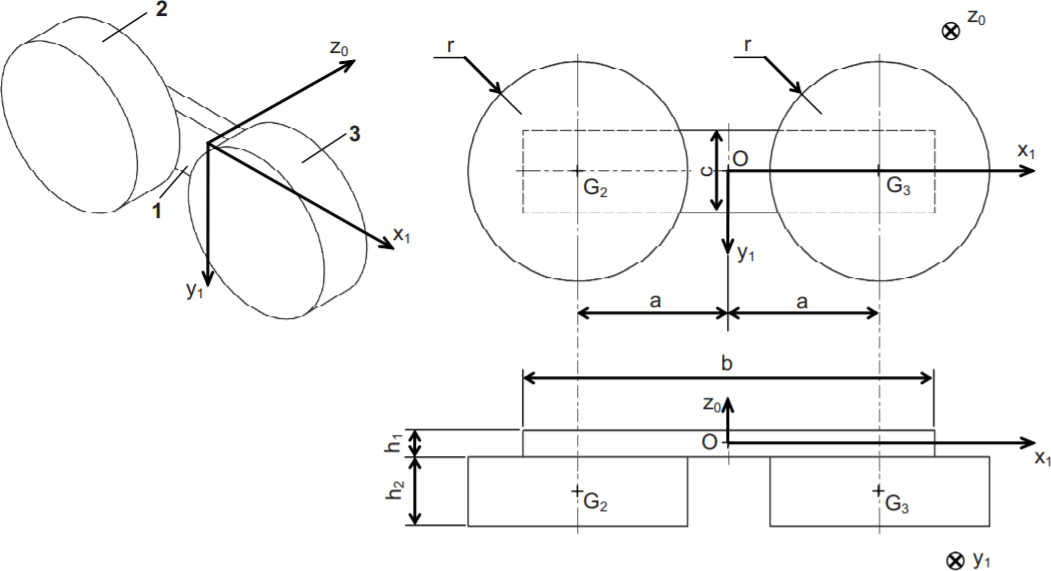
\includegraphics[width=\linewidth]{65_01}
\end{center}

$H_L(p)=\dfrac{K_L}{1+\tau_L p}$ et $H_G(p)=\dfrac{K_G}{1+\tau_G p}$  avec $\tau_G=\tau_L = \SI{20}{ms}$, $K_L = \SI{1e-3}{N^{-1}s^{-1}}$ et $K_G = \SI{2e-5}{mN^{-1}s^{-1}}$.


Le cahier des charges donne les valeurs des critères d'appréciation adoptés :
\begin{itemize}
\item la précision : en régime permanent à vitesse constante, soit $\varepsilon_S=0$ et à accélération constante, soit $\varepsilon_T=0$; $\varepsilon_S$ désigne l'erreur statique de position et $\varepsilon_T$ l'erreur statique de vitesse ou erreur de traînage;
\item la rapidité : le temps de réponse à \SI{5}{\%} tel que : $t_{\text{R}\SI{5}{\%}}\leq \SI{1}{s}$;
\item la stabilité : marge de phase $\geq \SI{45}{\degres}$ et marge de gain $\geq \SI{10}{dB}$.
\end{itemize}

On considère que le système n'est pas perturbé et que $T_G(p)=0$.
On choisit tout d'abord une correction intégrale telle que $C_V(p)=\dfrac{K_i}{p}$.

\question{Le cahier des charges est-il respecté en terme de précision ?}
\ifprof
\else 
\fi

\question{Calculer numériquement le temps de
réponse à \SI{5}{\%} optimal obtenu avec cette correction. Préciser la valeur de $K_i$ permettant d'obtenir ce temps de
réponse}
\ifprof
\else 
\fi

%\question{A-t-on augmenté ou diminué la rapidité du système par rapport à la correction proportionnelle ?}
%\ifprof
%\else 
%\fi

\question{Tracer l'allure du diagramme de Bode de la FTBO corrigée avec ce correcteur.}
\ifprof
\else 
\fi

\question{Indiquer la marge de phase.}
\ifprof
\else 
\fi

\question{Calculer la valeur de $K_i$ limite assurant le cahier des charges en terme de marge de phase.}
\ifprof
\else 
\fi

\question{Vérifier cette valeur en vous aidant du diagramme de Bode partiel de la fonction $C_V(p).H_L(p)$, donné  ci-dessous pour la valeur particulière : $K_i=7000$.}
\ifprof
\else 
\fi


\begin{center}
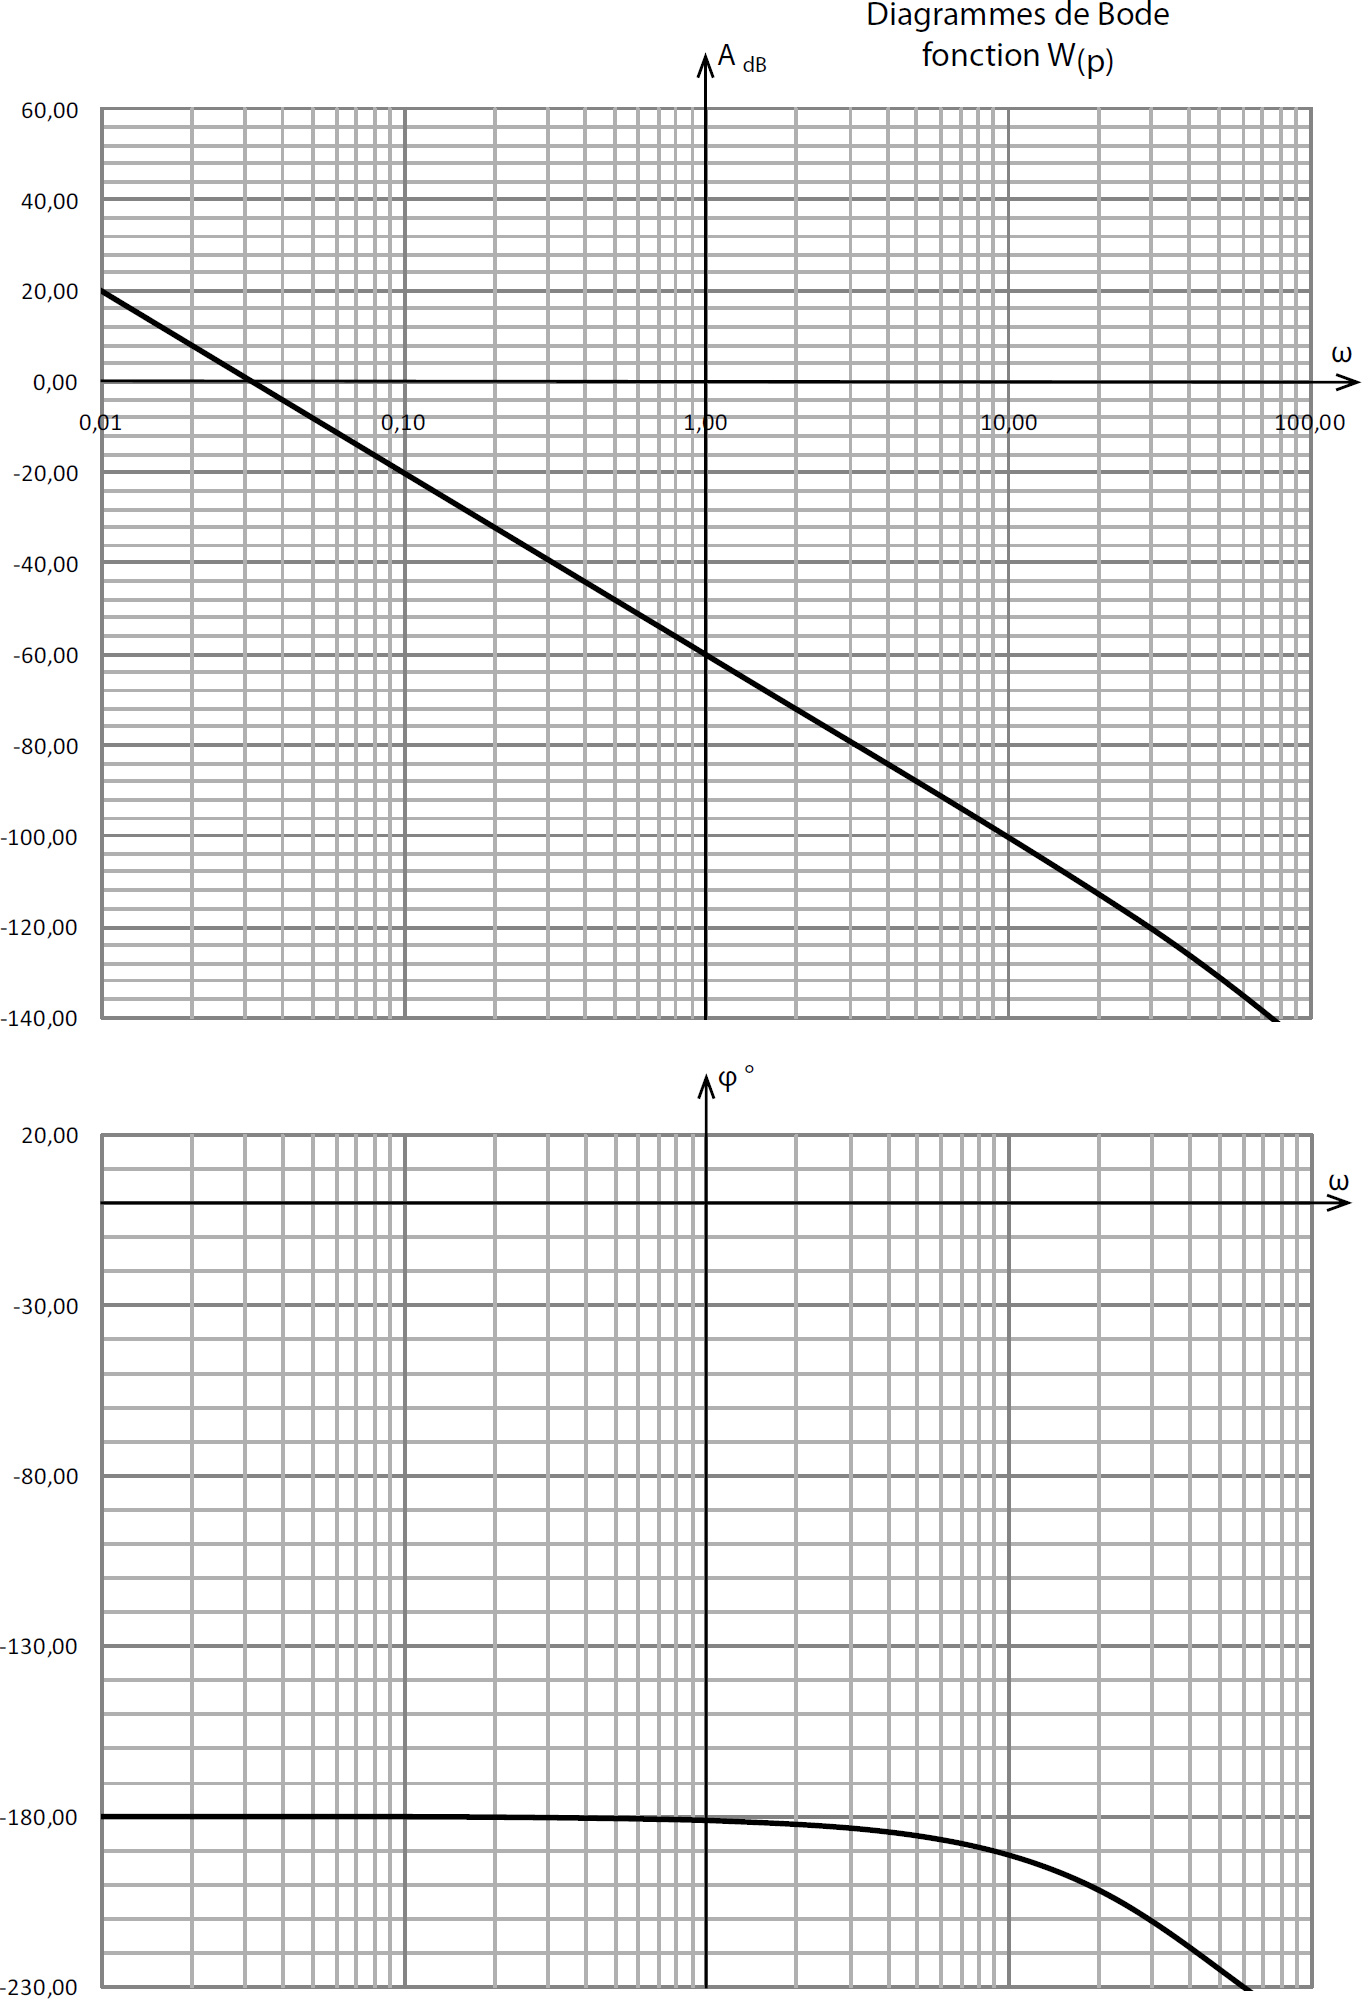
\includegraphics[width=\linewidth]{65_02}
\end{center}

\question{Que pensez vous de cette valeur, vis-à-vis du comportement du système, comparée à celle trouvée précédemment.}
\ifprof
\else 
\fi

\question{Un correcteur de type $C_V(p)=\dfrac{K_i}{p^2}$, permettrait-il d'obtenir les performances attendues en terme de précision et pourquoi ? }
\ifprof
\else 
\fi

\question{Permet-il d'assurer la stabilité du système et pourquoi ?}
\ifprof
\else 
\fi


\ifprof
\else

\noindent\footnotesize
% \fbox{\parbox{.9\linewidth}{
% Éléments de corrigé : 
% \begin{enumerate}
  % \item $\varepsilon_{\text{con \%}} = \dfrac{1}{1+K_PK_m K_{\text{pom}} K_{\text{cap}} }$;
  % \item $K_P > 19$;
  % \item $\varepsilon_{\text{pert}} = \Delta Q_e \dfrac{K_f}{1+K_{\text{cap}}K_PK_mK_{\text{pom}}}$;
  % \item $K_P > 2,19$.
  % \item $K_P < 0,125$. Il est impossible de vérifier les trois conditions avec un correcteur proportionnel.
% \end{enumerate}}}
\normalsize

\begin{flushright}
\footnotesize{Corrigé  voir \ref{C2:04:65:02}.}
\end{flushright}%
\fi